% Exemplo de relatório técnico do IC

% Criado por P.J.de Rezende antes do Alvorecer da História.
% Modificado em 97-06-15 e 01-02-26 por J.Stolfi.
% modificado em 2003-06-07 21:12:18 por stolfi
% modificado em 2008-10-01 por cll
% modificado em 2010-03-16 17:56:58 por stolfi
% modificado em 2012-09-25 para ajustar o pacote UTF8. Contribuicao de Rogerio Cardoso
% \def\lastedit{2015-03-18 00:52:20 by bit}

\nonstopmode % PARA RODAR LATEX EM BATCH MODE
\documentclass[11pt,twoside]{article}

\usepackage{techrep-ic}
\usepackage{amsmath}
\usepackage[english]{babel}
\usepackage[utf8]{inputenc}
\usepackage[margin=1in]{geometry}
\usepackage[
  style=numeric,
  sorting=none
]{biblatex}
\addbibresource{references.bib}
\usepackage[hidelinks]{hyperref}
\usepackage[noabbrev, capitalise]{cleveref}
\usepackage[cache=false]{minted}

\begin{document}

%%% PÁGINA DE CAPA %%%%%%%%%%%%%%%%%%%%%%%%%%%%%%%%%%%%%%%%%%%%%%%
% 
% Número do relatório
\TRNumber{41} % Dois dígitos
\TRYear{23} % Dois dígitos
\TRMonth{12} % Numérico, 01-12
\TRAuthor{Paulo Pacitti \and Julio López}
\TRTitle{Exploring ASCON\ on 64-bit RISC-V}
\TRMakeCover

%%%%%%%%%%%%%%%%%%%%%%%%%%%%%%%%%%%%%%%%%%%%%%%%%%%%%%%%%%%%%%%%%%%%%%
% O que segue é apenas uma sugestão - sinta-se à vontade para
% usar seu formato predileto, desde que as margens tenham pelo
% menos 25mm nos quatro lados, e o tamanho do fonte seja pelo menos
% 11pt. Certifique-se também de que o título e lista de autores
% estão reproduzidos na íntegra na página 1, a primeira depois da
% página de capa.
%%%%%%%%%%%%%%%%%%%%%%%%%%%%%%%%%%%%%%%%%%%%%%%%%%%%%%%%%%%%%%%%%%%%%%

%%%%%%%%%%%%%%%%%%%%%%%%%%%%%%%%%%%%%%%%%%%%%%%%%%%%%%%%%%%%%%%%%%%%%%
% Nomes de autores ABREVIADOS e titulo ABREVIADO,
% para cabeçalhos em cada página.
%
\markboth{Pacitti, López}{Exploring ASCON on 64-bit RISC-V}
\pagestyle{myheadings}
\thispagestyle{empty}

%%%%%%%%%%%%%%%%%%%%%%%%%%%%%%%%%%%%%%%%%%%%%%%%%%%%%%%%%%%%%%%%%%%%%%
% TÍTULO e NOMES DOS AUTORES, completos, para a página 1.
% Use "\\" para quebrar linhas, "\and" para separar autores.
%
\title{Exploring ASCON on 64-bit RISC-V}

\author{Paulo Pacitti\thanks{Computer Engineering Undergraduate, Institute of Computing, UNICAMP. \texttt{p185447@dac.unicamp.br}} \and
  Julio  López\thanks{Associate Professor, Institute of Computing, UNICAMP. \texttt{jlopez@ic.unicamp.br}}}
\date{}
\maketitle

%%%%%%%%%%%%%%%%%%%%%%%%%%%%%%%%%%%%%%%%%%%%%%%%%%%%%%%%%%%%%%%%%%%%%%

\begin{abstract}
  Sed quis lorem magna. Sed sit amet ullamcorper massa, sit amet placerat lectus. Suspendisse pulvinar ipsum sed enim commodo, ac malesuada lectus finibus. Aliquam eu eros eleifend, interdum nisi faucibus, viverra sapien. Vivamus lobortis a lectus eu rutrum.
  Quisque in est sit amet libero sollicitudin ornare a sed ipsum. Suspendisse potenti.
  Aliquam sit amet nisi sed nulla tincidunt imperdiet. Pellentesque elementum lacus eget
  dolor gravida lobortis. Sed placerat lacinia nisi, sed varius turpis facilisis ac.
\end{abstract}

\section{Introduction}
Inspired by the works of the UNICAMP's Laboratory of Security and Cryptography in the optimization of cryptographic algorithms for the ARM architecture \cite{Fujii2017a}, the NIST Lightweight Cryptography competition winner algorithm \cite{turan2023status}, and the RISC-V open architecture, this research aims to explore the Ascon family of algorithms \cite{asconv12nist} on the RISC-V 64-bit architecture and wether it's possible to optmize it for this architecture.

The approach was to analyze the Ascon algorithm design and 3 different implementations. All the implementations tested are written in C. The first implementation \texttt{ref} is the reference implementation of Ascon, written by Ascon team \cite{asconc2023}. The second one is \texttt{opt64}, and optmized implementation for a generic 64-bit architecture system, also developed by the Ascon team. The  third implementation was the main objective of this research, named \texttt{ascon-v} \cite{asconv2023}, this implementation is focused on producing a optmized version for the RISC-V 64-bit architecture. The research was focused on trying to improve the basic blocks of the Ascon family of algorithms. Because of that, the analysis, optimizations and results are focused on the \textsc{Ascon-128}, which is the \textit{de facto} AEAD standard of the Ascon family.

\section{Ascon}

Ascon is a family of algorithms for lighweight cryptography, designed to be used in constrained environments,
like embedding computing. Designed by cryptographers from Graz University of Technology, Infineon Technologies, Intel Labs, and Radboud University, Ascon has been selected as the new standard for lightweight cryptography in the 2019–2023 NIST Lightweight Cryptography competition. The Ascon family is mainly composed by 4 algorithms: \textsc{Ascon-128}, \textsc{Ascon-128a}, \textsc{Ascon-Hash} and \textsc{Ascon-Hasha}. There's also variants \textsc{Ascon-80pq}, \textsc{Ascon-Xof}, \textsc{Ascon-Xofa}, where the first it's a version of AEAD with an increased key size of 160 bits and the latter two are versions of the hash algorithm but they produce hash outputs of arbitrary
length, just changing the number of rounds necessary for it.

$$ \textrm{insert table with Ascon parameters} $$

Ascon lightweight properties comes from using the simple bitwise operations that majority of microcontrollers have, like XOR, AND, OR, NOT, and bitwise rotations. The algorithm is based on a sponge construction, which is a cryptographic primitive that can be used to build cryptographic hash functions, pseudorandom functions, and authenticated encryption schemes, like the SHA-3 (also know as "Keccak") \cite{bertoni2015keccak} algorithm. The sponge construct consists in keeping a finite internal state that takes input streams (absorb) to update the state and output streams (squeeze) to produce the output from the internal state, as it's displayed in \cref{fig:1}.

\begin{figure}[h]
  \centering
  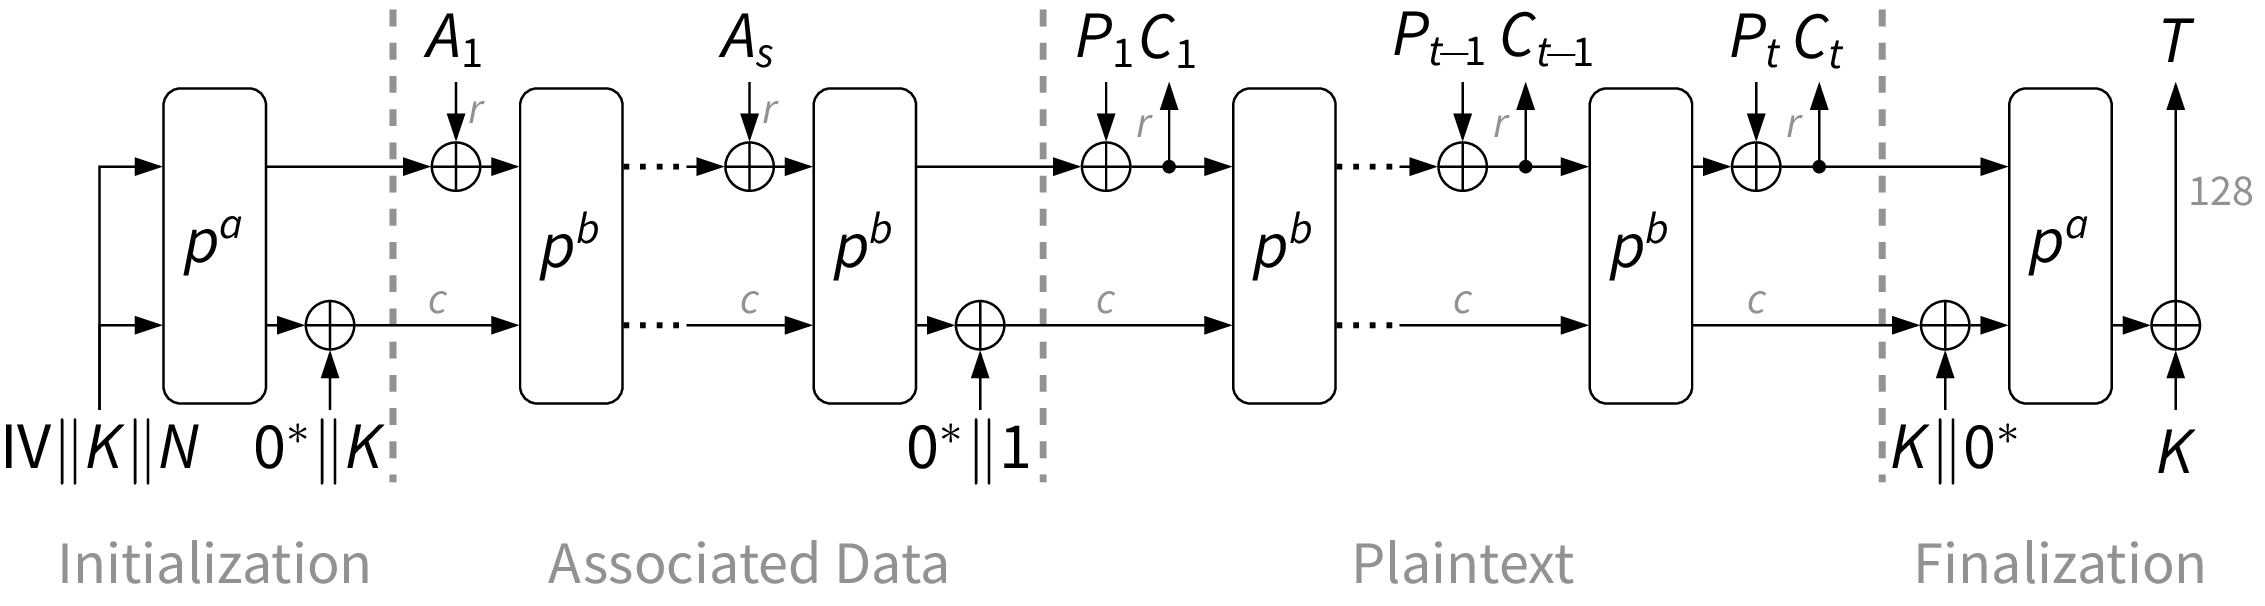
\includegraphics[width=.64\textwidth]{assets/aead_encrypt.png}
  \caption{Sponge construct for AEAD encryption with ASCON.}
  \label{fig:1}
\end{figure}


The Ascon state is composed by 5 64-bit words, alson named as Ascon words, resulting in a 320-bit internal state. This internal state is then manipulated using the Ascon permutation procedure.

\subsection{Permutation}

\subsection{Encryption}

\subsection{Decryption}

\section{RISC-V}

\section{Implementation}

The device used for this research is the MangoPi MQ-Pro, a SBC powered with a
Allwinner D1 chip and 1GB DDR3 of RAM, with Wi-Fi, Bluetooth and HDMI video
output. The Allwinner D1 chip contains a T-Head Xuantie C906 core, a RISC-V
64-bit 1GHz CPU supporting RV64GC ISA. The board runs Ubuntu Server 23.04,
running the 6.2.0-36-generic version of the Linux kernel. For compiling the implementation in C, it was used the RISC-V GNU Compiler Collection
(GCC) version 12.2.0 \cite{riscvgnutoolchainv2023} through cross-compilation with Newlib, using a MacBook Pro with an Apple M1 chip.

Ascon words, used to mantain the state in the sponge construct, are big endian. The reference implementation merges data to these words by loading and storing bytes using big-endianess, requiring operations to fill the right-side with zeros. However, RISC-V, as like most of other ISAs, is little endian, making bitwise operations slower than it could be if the architecture had the same endianess than the algorithm. It's possible to implement an opmitization considering this issue by handling the data as little-endian in the implementation and reversing the endianess when merging data to the Ascon words \cite{jellema2019optimizing}. This turns out to be way more effective than operating in data in big endinaness since loading bytes and other biwise operations does not need to fill the right-side of the bistring with zeros, as it is in big-endinaness. That way, the cost of reversing the endianess of little-endian 64-bit bistring is lower than the cost of loading data in big-endianess.

\section{Results}

Considering $t$ the elapsed time to run encryption/decryption of a plaintext/ciphertext, the resolution $R$ of the timer used to measure the time of the C906 core to be 45 nanoseconds  \cite{10179399}, $F$ the CPU frequency, the number of clock cycles used in encryption/decryption can be calculated \cref{eq:1}:

\begin{equation}
  C = t \times R \times F \times \frac{10^{9}}{60} \label{eq:1}
\end{equation}

\section{Future}
As we can see, the RV64GC instructions do not allow great optimizations from the architecture itself since it doesn't have any special instructions to accelerate operations of the Ascon128. However, RISC-V does have instructions extensions in development, and even ratfied, that could improve the performance of Ascon. Such cryptographic specialized instruction extenstions are divided in scalar and vectorial.

The Scalar Cryptography set of extensions (Zbkb, Zbkc, Zbkx, Zknd, Zkne, Zknh, Zksed, Zksh, Zkn, Zks, Zkt, Zk, Zkr) \cite{riscvCryptoVol1} provide instructions that could accelerate operations of the Ascon permutation.
The extension Zbkb provides bitmanipulation instructions for cryptographic operations having bit rotations operations, that could replace the rotation using two shift instructions in the Ascon permutation, as .

\begin{minted}{C}
// Ascon permutation
static inline uint64_t ROR(uint64_t x, int n) {
  return x >> n | x << (-n & 63);
}
\caption{Sponge construct for AEAD encryption with ASCON.}
\end{minted}

\section{Conclusions}

\printbibliography

\end{document}
